\documentclass[11pt]{beamer}
\usetheme{Warsaw}
\usepackage[utf8]{inputenc}
\usepackage{amsmath}
\usepackage{amsfonts}
\usepackage{amssymb}
\author{Team Expeditus}
\title{UAV Autonomous Landing}
%\setbeamercovered{transparent} 
%\setbeamertemplate{navigation symbols}{} 
%\logo{} 
\institute{Dept. of Computer Science, SDSMT} 
%\date{} 
%\subject{} 
\begin{document}

\begin{frame}
\titlepage
\end{frame}

%\begin{frame}
%\tableofcontents
%\end{frame}

\begin{frame}{Team}
\textbf{Team Expeditus}\\
Jonathan Dixon, Dylan Geyer, Christopher Smith, Steven Huerta\\ 
\vspace{6mm}
\textbf{Sponsor}\\
Dr. Larry Pyeatt\\
\vspace{6mm}
\textbf{Goal}\\
Software to autonomously take-off, navigate to set waypoints, return to launch pad, and land
\end{frame}

\begin{frame}{Phase Objectives}
\textbf{Phase I}
\begin{itemize}
\item Build UAV 
\item Flight Controller Operating Correctly
\item Simulation Environment Available
\end{itemize}
\vspace{5mm}
\textbf{Phase II}
\begin{itemize}
\item Autonomous landing ready for simulation
\item Autonomous landing ready for UAV
\end{itemize}
\end{frame}

\begin{frame}{Testing}
\textbf{Phase I}
\begin{itemize}
\item Manual Flight of UAV
\item Autonomous Flight of UAV 
\end{itemize}
\vspace{5mm}
\textbf{Phase II}
\begin{itemize}
\item Autonomous Landing in Simulation
\item Autonomous Landing of UAV
\item Autonomous Take-off, Navigation, and Landing of UAV
\end{itemize}
\end{frame}

\begin{frame}{Approach - UAV}
\begin{figure}
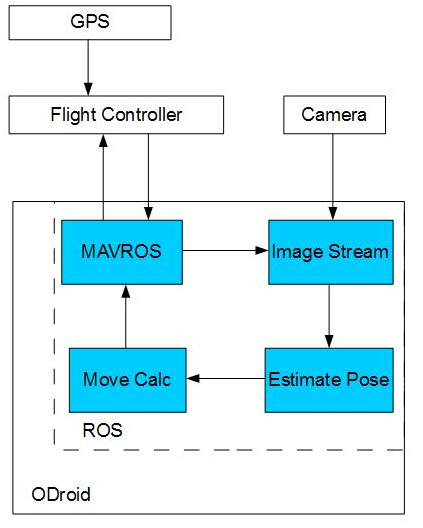
\includegraphics[width=.5\textwidth]{broad_approach1}
\end{figure}
\end{frame}

\begin{frame}{Approach - Landing Vision}
Put some stuff here about the landing vision approach, maybe a picture or two
\end{frame}

\begin{frame}{Approach - Landing AI}
Put some stuff here about the landing ANN approach, maybe a picture or two
\end{frame}


\begin{frame}{Development - Software}
List Software Here
\end{frame}

\begin{frame}{Development - Hardware}
List Hardware Here
\end{frame}

\begin{frame}{Cost}
Cost table of UAV purchase, maybe augmented a bit for neatness
\end{frame}

\begin{frame}{Work Accomplished}
List of Work Accomplished
\end{frame}

\begin{frame}{Risk}
List of Problems Encountered this first sprint
\end{frame}

\begin{frame}{Conclusion}
Conclusion-y stuff here
\end{frame}

\begin{frame}
\textbf{Questions?}
\end{frame}

\end{document}
